\documentclass[tikz,border=8pt]{standalone}
\usepackage[scaled=0.95]{helvet}
\renewcommand{\familydefault}{\sfdefault}
\usepackage{amsmath}
\usepackage{xcolor}
\definecolor{TEJNavy}{HTML}{1E2B55}
\definecolor{TEJOrange}{HTML}{E97828}
\definecolor{TEJRule}{HTML}{B8C2D1}
\begin{document}
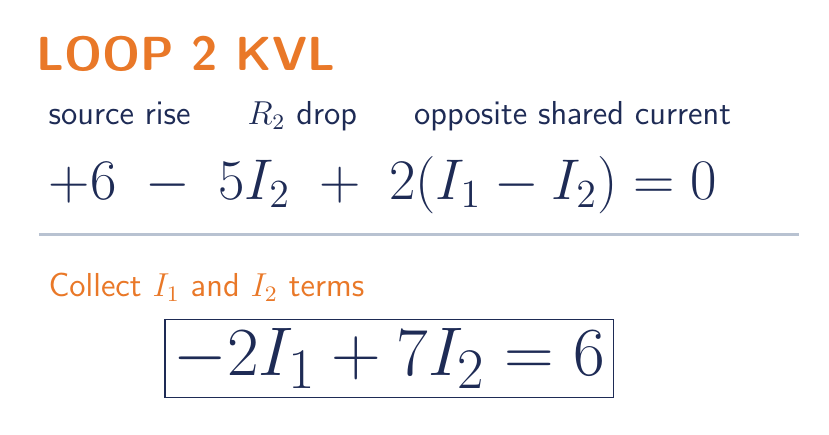
\begin{tikzpicture}[text=TEJNavy]
  \node[anchor=west,font=\bfseries\LARGE,text=TEJOrange] at (0,4.25) {LOOP 2 KVL};
  \node[anchor=west,font=\large] at (0.15,3.45)
    {source rise \hspace{0.45cm} $R_2$ drop \hspace{0.45cm} opposite shared current};
  \node[anchor=west,font=\huge] at (0.15,2.58)
    {$+6\; -\;5I_2\; +\;2(I_1-I_2)=0$};
  \draw[TEJRule,line width=1.2pt] (0.15,1.95) -- (9.8,1.95);
  \node[anchor=west,font=\large,text=TEJOrange] at (0.15,1.28)
    {Collect $I_1$ and $I_2$ terms};
  \node[anchor=west,font=\Huge] at (1.62,0.38)
    {$\boxed{-2I_1+7I_2=6}$};
\end{tikzpicture}
\end{document}
